\chapter{序論}
本研究にて,ユーザが定義した手書きジェスチャを高速に認識し,かつ容易に実装可能な軽量なアルゴリズムを示す.
本章にて,まず初めに研究背景として手書きジェスチャ認識の変遷及び既存の手書きジェスチャ認識手法とその課題を述べる.次にその課題を解決すべく本研究の目的を述べ,最後に本論文の構成を述べる.

\section{背景}
手書きジェスチャとは図\ref{fig:handwriting}のような,指やペンを用いた手書き動作を表し,その動作によって生成された軌跡あるいは文字や記号を認識することを手書きジェスチャ認識という.手書きジェスチャ認識を実現するための手法としてオンライン手書きジェスチャ認識がある.これは,
%アナログ行為である手書きを,情報処理可能なデータに変換するデジタル化のプロセスである.
タブレットなどに入力された手書きジェスチャの軌跡あるいは文字や記号において,時系列の筆点座標列から手書きジェスチャを自動認識する手法である.
このオンライン手書きジェスチャ認識による手書きジェスチャ認識は長年にわたり研究・開発され,多くのシステムに取り入れられてきた.

\begin{figure} [htbp]
\centering
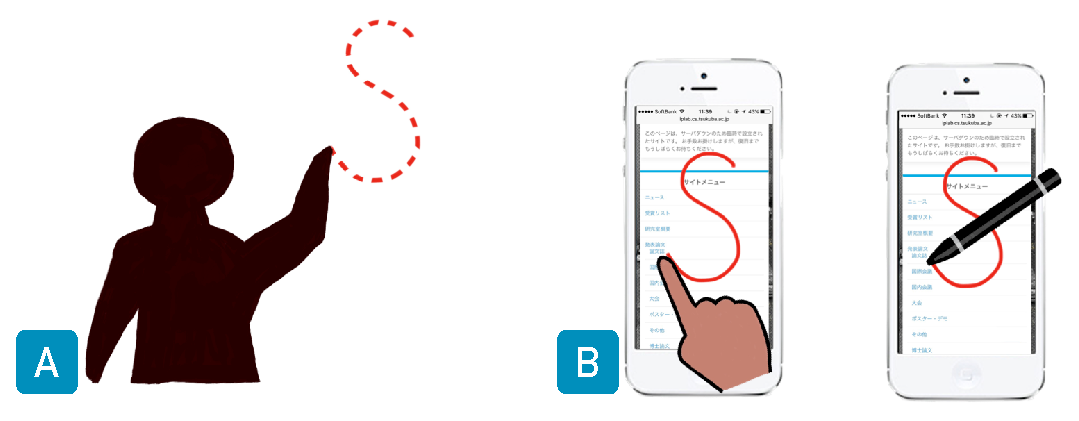
\includegraphics [width=0.5\columnwidth]{img/handwriting.eps}
\caption{手書きジェスチャの例.(A)空中にて指を用いて手書き動作する例.(B)スマートフォンに手書き動作をし,文字を入力する例.}
\label{fig:handwriting}
\end{figure}


その歴史は,
1964年のRANDタブレットにおいて英数字を認識することから始まる.
1970〜1980年代には日本語の文字認識も発表され,1984年には,松下電器から手書き文字認識を謳ったワープロが発売された.
1990年にはソニーがPalmtopを発表し,携帯PCにおいて,キーボードに代わる入力手段としてペン入力と手書き文字認識が採用された.
1991年にはGO社のPen Point オペレーティングシステムやMicrosoft Windows for Penが発売された.これらはペンPCと総称され,メーカー各社の手書き文字認識が搭載された.
しかしながら,実際使ってみると認識できない文字が多く存在したり,認識可能な記号を数十種類覚える必要があったりするなど多くの問題を抱えており,シェアは伸びなかった.
1993年には,Apple社がNewton,シャープがZaurusを発売し,PDAという新しい情報端末の概念が人気を博した.
%2004年に発売された任天堂のDSは,手書き認識の利用分野として20年間われ続けていた教育への利用を脳トレというコンセプトで結実させた.
そして,2007年にApple社から発売されたiPhoneは,直接操作,そして,書けるインタフェースとして広く普及した.
また,近年は電子ペーパーや電子書籍も普及してきており,手書きジェスチャ認識を用いたアプリケーションを搭載した端末は今後も開発され続けるであろう~\cite{110009437469}.

手書きジェスチャ認識が長年にわたり研究・開発されてきた理由は,手書きジェスチャ入力には以下に示す利点が存在するからである.
\begin{itemize}
 \item 人間にとって自然なインターフェースである
 
ペンで紙に書くという行為は、物事を伝えたり何かを表現したりすることにおいて,人間にとってもっとも自然な行為の1つである.
 \item 素早く入力できる
 
例えば,あるコマンドを実行する際に,ボタンにより遷移するUI(図\ref{fig:wallpaper}(A))よりも,文字や記号などを直接書き込むことにより実行できるようなUI(図\ref{fig:wallpaper}(B))の方が早く操作できる.また,英字などを入力する場合(図\ref{fig:keyinput})においては,特にスマートフォンのようにキーボードの領域が小さい場合は,手書き入力の方が早く入力できるうえ,画面を見ることなく入力することができる.

\begin{figure} [htbp]
\centering
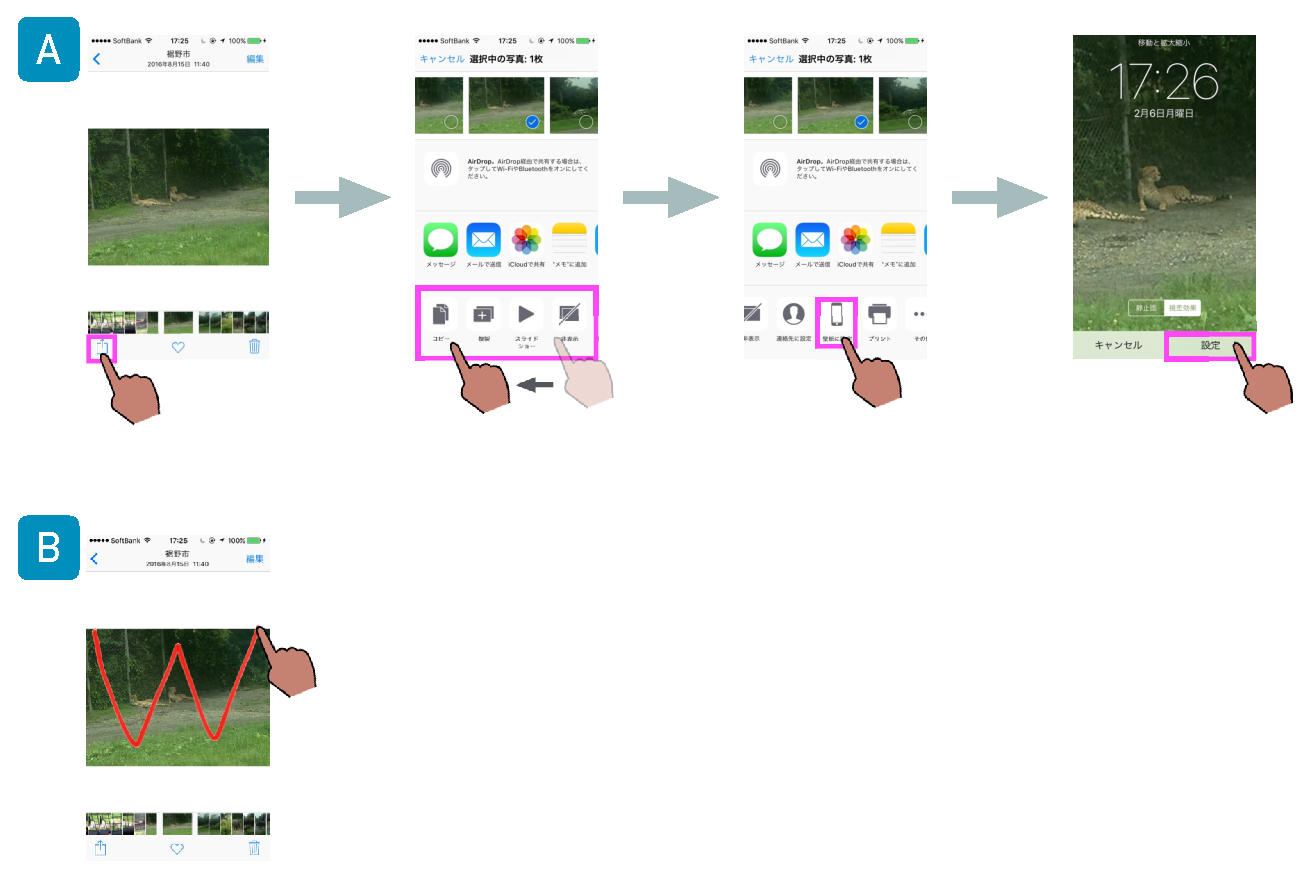
\includegraphics [width=0.85\columnwidth]{img/wallpaper.eps}
\caption{スマートフォンにおける壁紙を設定する例.ボタンにより遷移するUI(A)の場合,4ステップ必要であるが,文字や記号などを直接書き込むUI(B)の場合,1ステップにより設定することができる.}
\label{fig:wallpaper}
\end{figure}

\begin{figure} [htbp]
\centering
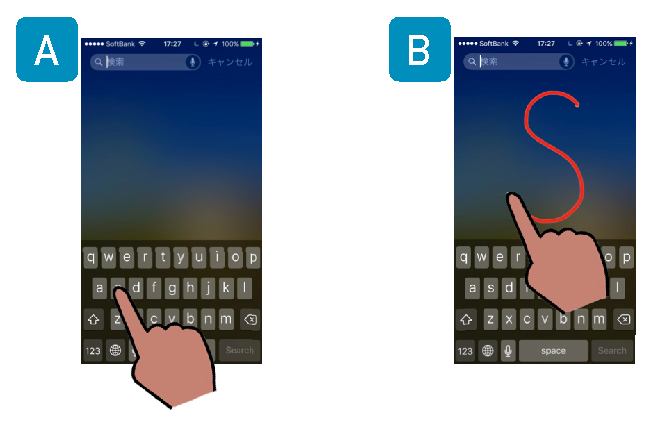
\includegraphics [width=0.5\columnwidth]{img/keyinput.eps}
\caption{キーボードにより入力する場合(A)は,操作領域が小さいため,入力に多くの時間を要したり誤って入力したりする場合がある.手書き入力の場合(B)は,操作領域が大きいため誤入力が生じづらい.また,画面を見ることなく入力可能である.}
\label{fig:keyinput}
\end{figure}

 \item 実際の操作の意味に紐づく入力ができる
 
 図\ref{fig:semantic}に示すように,「決定」操作をチェックマークに割り当てたり,「ヘルプ」操作をはてなマークに割り当てたりすることにより,実際の操作の意味に紐づく入力ができ,ボタンにより遷移するUIよりも,直感的に操作できる.
\end{itemize}

\begin{figure} [htbp]
\centering
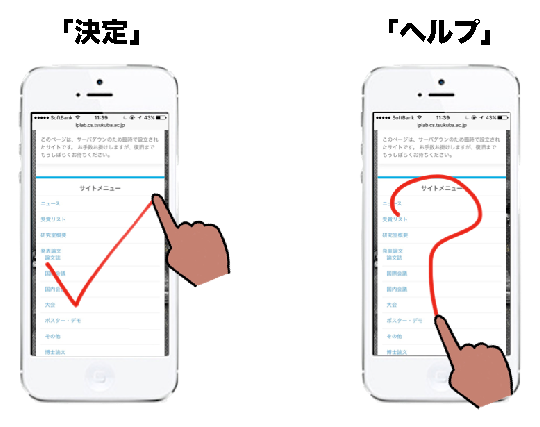
\includegraphics [width=0.5\columnwidth]{img/semantic.eps}
\caption{(A)「決定」操作にチェックマークに割り当てる例.(B)「ヘルプ」操作をはてなマークに割り当てる例.}
\label{fig:semantic}
\end{figure}

このような手書きジェスチャ入力の利点及び,近年にみるタッチパネルを搭載したスマートフォンやタブレット端末の普及により,手書きジェスチャ入力を用いたアプリケーションが多く開発されている.

特に手書きジェスチャ認識を用いたアプリケーションをプロトタイピングする環境において,手書きジェスチャをアプリケーションに組み込む際に求められることは~\cite{Rettig:1994:PTF:175276.175288}において以下のようなことが述べられている.
\begin{itemize}
 \item 複雑な数式やアルゴリズムを用いていない

ライブラリが提供されていないようなプロトタイピング開発環境においては,自分で実装するために,手書きジェスチャ認識を実現するためのパターン認識に関する専門的な知識~\cite{Hong00constructingfinite, Anderson2004HiddenMM,Sezgin:2005:HES:1040830.1040899, Cao:2005:EOA:1089508.1089540, Pittman:1991:RHT:108844.108914, Cho:2006:NGR:1711617.1711649,Rubine:1991:SGE:127719.122753, Anthony:2010:LMR:1839214.1839258}がなくとも,素早く実装できることが重要である.
また,認識率を向上させるなど,アルゴリズムを改善する場合においても,アルゴリズムが簡潔であることが求められる.

\item 少ない学習データにより認識できる

ジェスチャ認識を実現するためには,ほとんどの場合,開発者は膨大な数の学習データを用意する必要がある.
プロトタイピング開発環境においては,素早く手書きジェスチャ入力のテストができることが重要であり,そのために,少ない学習データにより認識できることが重要である.また,少ない学習データにより認識できるということは,アプリケーションユーザが独自に手書きジェスチャを定義することが可能なシステムを実現することにもつながり,これも手書きジェスチャを入力として用いるアプリケーションを開発する多くの開発者によって求められていることの1つである.

\item 認識率が高い,認識速度が速い

手書きジェスチャを入力として用いる場合,入力された手書きジェスチャの認識率が高いこと,入力してから認識されるまでの速度が速いことは,ユーザビリティ(使いやすさや使い勝手)の観点より重要である.

\item ロバスト性が高い

手書きジェスチャは,入力されるジェスチャの形状が毎回異なるため,たとえ形状が異なったとしても意図したジェスチャとして正しく認識されるようなロバスト性の高いアルゴリズムであることも重要である.
\end{itemize}

これらの要件を満たす手書きジェスチャ認識アルゴリズムとして,\$1~\cite{Wobbrock:2007:GWL:1294211.1294238}があげられる.このアルゴリズムは,「アルゴリズムが簡潔である,少ない学習データにおいて高い認識率を示す,認識速度が速い,ロバスト性が高い」といった特徴を持ち,単一ストロークな(一筆書きな)手書きジェスチャを認識可能なアルゴリズムである.アルゴリズムが簡潔であるため,ActionScript,Python,C\#,C++,Objective-C,Java,Java ME,JavaScriptといった言語において実装されている.
そのため,多くの開発者にとって,手書きジェスチャ認識を自身のシステムに組み込むことが容易となった.
また,上記に示す開発言語が利用できないようなプロトタイピング開発環境においても,アルゴリズムが簡潔ゆえ実装の敷居が低く,そのような環境において\$1の存在価値は高い.

\$1を改良した多くのアルゴリズムは\$-Family Recognizer~\cite{Anthony:2010:LMR:1839214.1839258,Reaver:2011:MQU:2021164.2021183,Li:2010:PFA:1753326.1753654,Anthony:2012:NFA:2305276.2305296,Herold:2012:CRF:2331067.2331074,Vatavu:2012:GPC:2388676.2388732,Taranta:2015:PPB:2788890.2788925,Pittman:2016:FFA:2856767.2856808,Vatavu:2012:OAF:2166966.2167022}として知られている.これらの\$-Family Recognizerは,\$1の持つ「アルゴリズムが簡潔である」という特徴を維持しつつ,認識率や認識速度の向上,識別可能なジェスチャの種類の増加という点において改良されており,今もなお.アルゴリズムの開発・改良の機運が高まっている.
%ペンや指を入力として用いるようなインタフェースが普及し,それらを用いたアプリケーションの開発者が増加している今日において,
%これらのアルゴリズムは,手書きジェスチャ認識を自身のシステムに容易に組み込むための手段として必要とされており,アルゴリズムの開発・改良の機運が高まっている.

これまで開発されてきた\$-Family Recognizerは,ジェスチャを構成するストロークの,大きさ,向き,位置に関して,そのいずれかあるいはすべてについて不変になるようなアルゴリズムを採用することにより,不変にしたものについてロバストなジェスチャ認識を実現した.大きさ,向き,位置に関して不変にするということは,手書きジェスチャの書き順が同じでありかつ手書きジェスチャの形状さえ類似していれば,ジェスチャの大きさ,向きあるいはジェスチャが入力された位置などが異なっても,同じ形状と書き順の手書きジェスチャとして認識されるということである.%その結果,認識率の向上が実現された.
一方,それらを不変にしない,つまり特徴量として認識のために用いるということは,その特徴量について識別できるため,識別可能な手書きジェスチャが増加することにつながるが,不変にしない特徴量についてはロバストではなくなるため,認識率の低下を招く恐れがある.
例えば,Rubine Classfier~\cite{Rubine:1991:SGE:122718.122753}は13もの手書きジェスチャの特徴量を用いることにより手書きジェスチャを認識し,手書きジェスチャを構成するストロークの形状と書き順は同じであるが,大きさ,向き,位置が異なるジェスチャ(図\ref{fig:examples_V})を識別することが可能である.
しかしながら,入力されるジェスチャの形状が毎回異なる手書きジェスチャにおいて,認識に用いる特徴量が多いことは,類似度が低くくなる特徴量が増える可能性が高くなることにつながり,結果的に認識率の低下を招いている.

\begin{figure} [htbp]
\centering
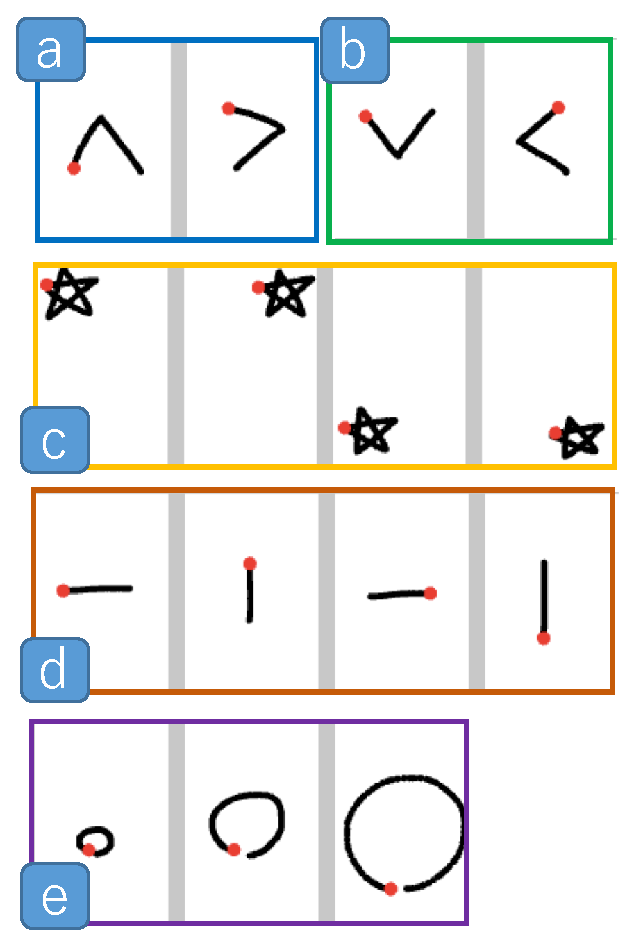
\includegraphics [width=0.5\columnwidth]{img/examples_V.eps}
\caption{ジェスチャの形状と書き順は同じであるが,向き (a)(b)(c),位置(d),大きさ(e)が異なる,単一ストロークからなる手書きジェスチャの例.}
\label{fig:examples_V}
\end{figure}

DTW~\cite{Tappert:1982:CSR:1664966.1664979, Salvador:2007:TAD:1367985.1367993}は,手書きジェスチャ認識を実現するために広く採用されているアルゴリズムである.
入力データと学習データにおいて,ストロークを構成する点の距離を比較するのみであるため,こちらも,手書きジェスチャを構成するストロークの形状と書き順は同じであるが,大きさ,向き,位置が異なるジェスチャを識別することは可能である.
ストロークを構成するすべての点に対し距離が最小となる点を全探索するため,アルゴリズムは単純であり,かつ認識率も高いが,計算量が大きいという問題点がある.
このように,手書きジェスチャを構成するストロークの形状と書き順は同じであるが,大きさ,向き,位置が異なるジェスチャを識別する場合,認識率及び認識速度双方において高い性能を示すことは難題である.

しかしながら,手書きジェスチャ入力に関するユーザ調査により,これまでに述べたきたような,ジェスチャの形状と書き順は同じであるが,大きさや向きや位置が異なる単一ストロークからなる手書きジェスチャ~(図\ref{fig:examples_V})をアプリケーションユーザが入力として用いることを要望していることが導かれた.
既に述べたように,これらの手書きジェスチャは,既存の\$-Family Recognizerにおいては識別できないため,ユーザが定義するこれらのような手書きジェスチャを入力として用いるようなアプリケーションを開発したい開発者は既存の\$-Family Recognizerを認識アルゴリズムとして用いることができない.また,これらを識別可能なRubine classfierやDTWを採用した場合は,認識率や認識速度において十分な性能を得られない可能性がある.


\section{目的}
本研究の目的は,\$1を拡張し,単一ストロークからなる手書きジェスチャに対し,ジェスチャの大きさ,向き,位置に関して識別可能としながらも,\$1と比較し認識率の低下と認識速度の低下を抑えることを実現した\$-Family Recognizer開発することである.
我々はこの,ジェスチャの大きさ,向き,位置に関して``V''ariant(異なる)手書きジェスチャを認識する\$-Family Recognizerを\$Vと名付けた.
\$Vは\$1に簡単な数式からなるアルゴリズムを追加することによって,どのような開発環境においても実装可能なアルゴリズムを開発することも目標としている.
また,\$1と同様,少ない学習データにおいて高い認識率を示すことも目標としており,これは,アプリケーションユーザが手書きジェスチャを独自に定義することが可能であることを示している.
また,大きさ,向き,位置に関して識別可能な既存アルゴリズムと比較することによって,\$Vの有用性を示すことも本研究における目的とする.


%\$Vは,大きさ,向き,位置を特徴量として用いることによって,それらに依存するストロークを識別可能とした.
%その際,学習データを元に,ストロークを形状と書き順ごとに分類し,認識に用いる特徴量に重み付けをすることによって考慮すべき特徴量を適切に配分し,\$1と比べても遜色のない認識率と認識速度を実現した.
%\$1を改良した多くのアルゴリズムを用いず,\$1を拡張した理由は,\$1にて計算された,大きさ,向き,位置の特徴量を再利用することによって,\$1アルゴリズムと比べて,アルゴリズムの追加量を抑えること,認識速度の低下を抑えることにつながるからである.

\section{貢献}
本研究における手書きジェスチャ認識アルゴリズム\$Vの貢献を以下に示す.
\begin{itemize}
\item 手書きジェスチャを構成するストロークの形状と書き順は同じであるが,大きさ,向き,位置に関して異なる手書きジェスチャを識別することが可能なアルゴリズムを開発した.
\item 少ない学習データにおいて認識率を向上させるためのアルゴリズムを開発した.
\item 認識速度を向上させるためのアルゴリズムを開発した.
\item 実装が容易な軽量なアルゴリズムを開発した.
\end{itemize}

\section{本論文の構成}
第1章では,研究背景と目的を述べた.第2章では,関連研究を述べる.第3章では,本研究の動機となった,手書きジェスチャ入力に関する調査を述べる.第 4 章では,\$Vの拡張元である\$1アルゴリズムを述べ,第5章において,\$Vのアルゴリズムの詳細を述べる.第6章では,\$Vのアルゴリズムとしての性能評価実験を述べる.第7章では,\$Vのアプリケーション例を述べる.第8章では,\$Vアルゴリズムの改善点と今後の展望を議論する.第9章では,本研究の結論を述べる.
なお,付録 A に\$Vアルゴリズムの擬似コードを示す.
%付録 B に第 3章のユーザ調査に用いた調査同意書を,付録 B に調査について説明する際に用いた説明書を,付録 Dに第6章の評価実験に用いた実験同意書を示す.
